\setlength{\columnsep}{3pt}
\begin{flushleft}
	
\begin{itemize}
	\item The organizational structure inside a partition is called \textbf{filesystem}.
	\item Once a partition is created, it should be given a \textbf{filesystem} to make the partition ready to use.
	\item The first Linux operating systems used the \textbf{extended (i.e ext) filesystem }.
\end{itemize}

\begin{figure}[h!]
	\centering
	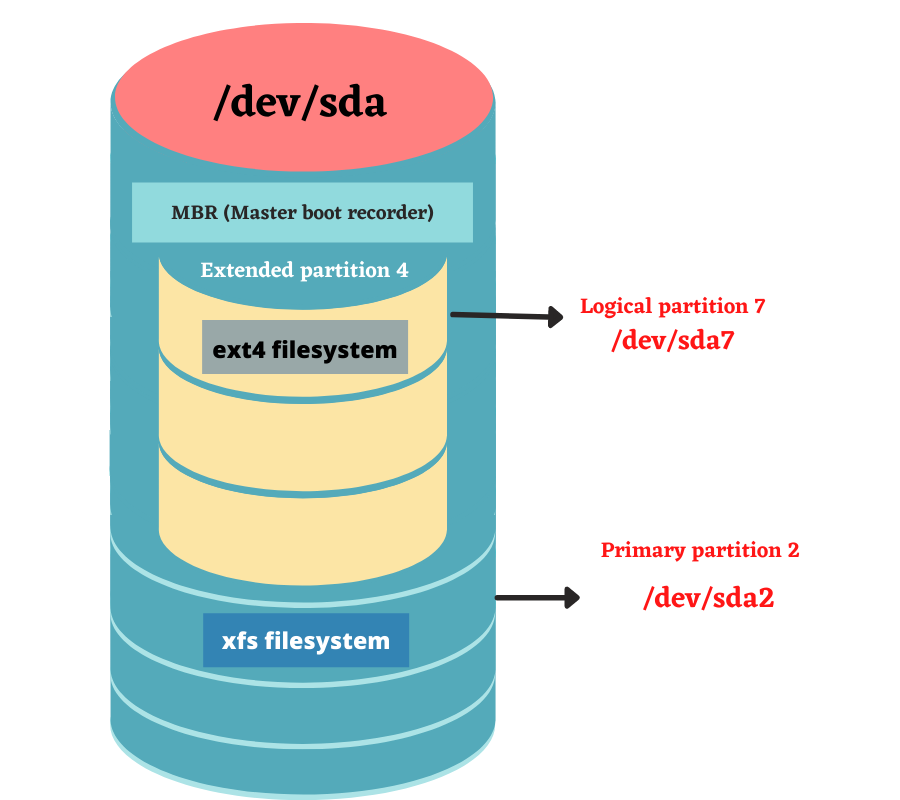
\includegraphics[scale=.6]{content/chapter8/images/newfilesystem.png}
	\caption{Filesystem}
	\label{filesystem}
\end{figure}

\begin{tcolorbox}[breakable,notitle,boxrule=1pt,colback=yellow,colframe=yellow]
	\color{black}
	Note: Without applying filesystem, the partitions of HDD should not be used.
\end{tcolorbox}


\newpage
\paragraph{Filesystem types}
\bigskip
\begin{tabulary}{1.0\textwidth}{|p{5em}|p{23em}|}
	\toprule
	\textbf{Type} & \textbf{Filesystem description}\\
	\midrule
	ext & 
	\begin{itemize}
		\item First Linux filesystem
	\end{itemize}
	\\
	\hline
	ext2 & 
	\begin{itemize}
		\item Second extended filesystem
		\item Maximum size of partition can be 32TB
		\item Maximum file size can be 2TB
	\end{itemize}
	\\
	\hline
	ext3 & 
	\begin{itemize}
		\item Third extended filesystem
		\item Maximum size of partition can be 32TB
		\item Maximum file size can be 2TB
		\item Journaling option available
	\end{itemize}
	\\
	\hline
	ext4 & 
	\begin{itemize}
		\item Fourth extended filesystem
		\item Maximum size of partition can be 1PB
		\item Maximum file size can be 16TB
		\item Journaling option available
		\item Defragmentation option available
	\end{itemize}
	\\
	\hline
	xfs &  
	\begin{itemize}
		\item High-performance 64-bit journaling filesystem
		\item Maximum file size and partition size can be 8EB (exbibytes)
		\item Maximum number of files that can be created are 264
	\end{itemize}
	 \\
	\bottomrule
\end{tabulary}
\newpage
\begin{tcolorbox}[breakable,notitle,boxrule=1pt,colback=pink,colframe=pink]
	\color{black}
	What is journaling filesystem?
	\begin{itemize}
		\item Journaling provides fault tolerance in file systems.
		\item It keeps track of all changes in a log before saving it to the HDD.
		\item Journaling helps in recovering system crashes and power failures.
		\item Permanent data loss is avoided.
	\end{itemize}
\end{tcolorbox}

\bigskip
\begin{tcolorbox}[breakable,notitle,boxrule=1pt,colback=pink,colframe=pink]
	\color{black}
	What is defragmentation in filesystem?
	\begin{itemize}
		\item Defragmentation makes sure unused space on the hard disk is all together.
	\end{itemize}
\end{tcolorbox}


\newpage

\paragraph{Command to apply filesystem on a partition}
\textbf{mkfs}: Stands for \textbf{Make Filesystem}. It applies a filesystem on a partition of HDD, USB drive, etc.

\bigskip
\begin{tcolorbox}[breakable,notitle,boxrule=-0pt,colback=pink,colframe=pink]
	\color{black}
	\fontdimen2\font=1em
	Syntax: mkfs -t filesystem\_name device\_name
	\fontdimen2\font=4pt
\end{tcolorbox}

Eg: Apply \textbf{"xfs"} filesystem on partition /dev/sdb1:
\begin{tcolorbox}[breakable,notitle,boxrule=-0pt,colback=black,colframe=black]
	\color{green}
	\fontdimen2\font=1em
	\# mkfs -t xfs /dev/sdb1
	\fontdimen2\font=4pt
\end{tcolorbox}

\bigskip
\bigskip

\paragraph{Filesystem UUID}

Once you have applied a filesystem to a partition, it is alotted with a \textbf{universally unique identifier} called as \textbf{UUID}. 

\newline
Command to check \textbf{UUID} of all filesystem:

\bigskip
\begin{tcolorbox}[breakable,notitle,boxrule=-0pt,colback=pink,colframe=pink]
	\color{black}
	\fontdimen2\font=1em
	Syntax: blkid
	\fontdimen2\font=4pt
\end{tcolorbox}

Eg:
\begin{tcolorbox}[breakable,notitle,boxrule=-0pt,colback=black,colframe=black]
	\color{green}
	\fontdimen2\font=1em
	\# blkid
	\newline
	\color{white}
	/dev/sdb1: PARTUUID="4f7c2ba4-01"
	\newline
	/dev/sda1: UUID="cd73be54-75ea-4705" TYPE="ext4"
	\newline
	/dev/sda2: UUID="7db79e4a-5144-43c4" TYPE="swap"
	\fontdimen2\font=4pt
\end{tcolorbox}

\end{flushleft}
\newpage

